\pagebreak
\section{Cursograma de Cobranzas}
La empresa posee distintas formas de cobros, las cuales varian con el cliente. Algunas clientes pagan a traves de una cuenta corriente con una transferencia, otros con cheque o efectivo. A determinados clientes se les envía un cobrador mientras que muchos otros no.
Por simplicidad, en este caso se describe el caso en el cual el cliente se acerca a la empresa al sector de finanzas a entregar los valores (cheques o efectivo).

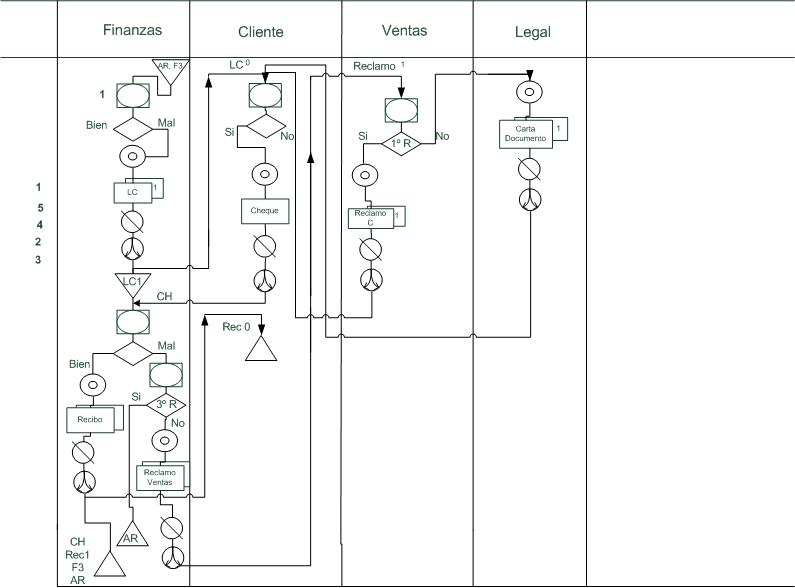
\includegraphics[scale=0.7]{Empresa/Circuitos/Cobranzas/cursograma-manual-cobranzas.jpg}

\pagebreak
\section{Procedimiento de Cobranzas}
\begin{enumerate}
  \item \textbf{Finanzas:} ejecuta un reporte en el sistema, el cual trae todas las facturas que vencen a la fecha. De ellas selecciona aquellas que no han sido pagadas. Esta tarea se realiza todos los días.
  Por cada factura vencida que no este paga, emite un reclamo del pago por duplicado, con una fecha de vencimiento de pago. El primero lo firma y se lo envía al cliente. El otro lo archiva para que quede constancia del reclamo.
  \item \textbf{Cliente:} recibe el reclamo o carta de documento, y en caso de pagar, confecciona un cheque para realizar el mismo y lo envia al sector de finanzas.
  \item \textbf{Finanzas:} en caso de recibir el cheque, revisa que corresponda con la cantidad a pagar y que este correctamente confeccionado. Si este esta correcto, emite un recibo por duplicado, firma el original y se lo entrega al cliente. Finalmente, archiva el cheque, la factura por triplicado, el duplicado del reclamo y registra en el sistema el pago de la factura.
  Si el cliente no paga, emite un reclamo a ventas y se lo envia a dicho sector. Si ya es la tercera vez que el cliente no paga, archiva los documentos utilizados y asienta en el sistema la falta de pago en la cuenta "pérdidas".
  \item \textbf{Ventas:} recibe el reclamo y si es la primera vez que se recibe un reclamo emite un segundo reclamo al cliente por duplicado. Firma el original y lo envia al cliente con una fecha límite para el pago. Si no es la primera vez que recibe un reclamo de finanzas, avisa de al sector legal de la falta de pago del cliente de manera informal(mail, llamado telefónico).
  \item \textbf{Legal:} una vez notificado de la falta de pago del cliente, emite una carta de documento, intimando al cliente a pagar las facturas que debe. La carta de documento es enviada al domicilio legal del cliente de forma tal que quede notificado.
\end{enumerate}

\pagebreak
\section{Manual del Cursograma de Cobranzas}

\begin{center}\textbf{Sectores intervinientes}\end{center}
\begin{itemize}
  \item Finanzas
  \item Ventas
  \item Cliente
  \item Legal
\end{itemize}

\begin{center}
  \textbf{Documentos}
  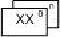
\includegraphics{./Images/Simbolos/simbolo-Documentos.png}
\end{center}
\begin{enumerate}
\item Reclamo a Cliente
\item Reclamo a Ventas
\item Cheque
\item Recibo
\item Carta Documento
\end{enumerate}

\begin{center}
  \textbf{Emisión de Documentos}
  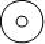
\includegraphics{./Images/Simbolos/simbolo-Emision-de-Documentos.png}
\end{center}
\begin{enumerate}
\item Finanzas: Emite primer Reclamo a Cliente por original y copia.
\item Finanzas: Emite Recibo por original y copia.
\item Finanzas: Emite Reclamo a Ventas.
\item Cliente: Emite Cheque.
\item Ventas: Emite segundo y tercer Reclamo a Cliente por original y copia.
\item Legal: Emite Carta Documento por original y copia.
\end{enumerate}

\begin{center}
  \textbf{Firma}
  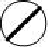
\includegraphics{./Images/Simbolos/simbolo-Firma.png}
\end{center}
\begin{enumerate}
\item Finanzas: Firma el original del primer Reclamo a Cliente.
\item Finanzas: Firma recibo oringinal con la entrega del cheque.
\item Finanzas: Firma el Reclamo a Ventas y se lo envia a dicho sector.
\item Cliente: Firma el cheque que luego entrega contra recibo a Finanzas.
\item Ventas: Firma el original del segundo o tercer Reclamo a Cliente.
\item Legal: Firma original de Carta Documento con la que notifica al cliente de la falta de pago.
\end{enumerate}

\begin{center}
  \textbf{Distribución}
  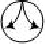
\includegraphics{./Images/Simbolos/simbolo-Distribucion.png}
\end{center}
\begin{enumerate}
\item Finanzas: distribuye el original del primer Reclamo a Cliente al cliente y conserva el duplicado.
\item Finanzas: entrega el recibo original a cambio del cheque recibido y conserva el duplicado del recibo.
\item Finanzas: distribuye el Reclamo a Ventas al sector de Ventas.
\item Cliente: entrega el cheque contra recibo.
\item Ventas: distribuye el original del segundo o tercer Reclamo a Cliente al cliente y conserva el duplicado.
\item Legal: Firma el original de Carta Documento y conserva el duplicado.
\end{enumerate}

\begin{center}
  \textbf{Almacenamiento Transitorio}
  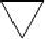
\includegraphics{./Images/Simbolos/simbolo-Almacenamiento-Transitorio.png}
\end{center}
\begin{enumerate}
\item Finanzas: almacena copia del primer Reclamo a Cliente.
\end{enumerate}

\begin{center}
  \textbf{Control y verificación}
  
\includegraphics{./Images/Simbolos/simbolo-Control-y-Verificacion.png}
\end{center}
\begin{enumerate}
\item Finanzas: Ejecuta un reporte en el sistema donde saca las facturas ya vencidas que no estan pagas. Controla el resultado del mismo con las factura por triplicado que tiene archivadas.
\item Finanzas: Verifica que el cheque que le fue entregado por el Cliente este correctamente confeccionado y se corresponda con el monto que indica la factura por triplicado que posee.
\item Finanzas: Luego de un tiempo controla si el Cliente pago o no el reclamo correspondiente. Verifica si el ya es el tercer reclamo que se le hizo al cliente.
\item Cliente: Verifica que sea correcta la factura que se le esta reclamando, y que se corresponda con lo que el mismo posee en sus registros y documentos.
\item Ventas: Ventas verifica si es el primer o segundo reclamo que le ha llegado por parte de una misma factura de ese cliente.
\end{enumerate}

\begin{center}
  \textbf{Decisión}
  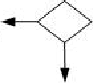
\includegraphics{./Images/Simbolos/simbolo-Decision.png}
\end{center}
\begin{enumerate}
\item Finanzas: Una vez que el resultado del reporte de facturas vencidas y que estas esten correctas emite los correspondientes reclamos para el cliente. Si no, no hace nada ( no hay facturas a cobrar).
\item Finanzas: Si el cheque recibido esta bien hecho y se corresponde con el monto de la factura vencida, procede a emitir el recibo correspondiente. Si el cliente no paga, venciendose el plazo de la factura o reclamo, procede a verificar si ya se han emitido otros reclamos o no.
\item Finanzas: Si ya era el tercer reclamo que se le envio al cliente, procede a asentar la falta de pago en el sistema. Si no, emite el primer o segundo reclamo correspondiente a Ventas.
\item Cliente: Una vez verificada la factura que se le reclama decide en caso de estar correcta la misma, confeccionar el cheque para realizar el pago. En caso contrario no hace nada (o depende de cada cliente, en realidad no interesa que hace si no paga).
\item Ventas: Una vez verificado el reclamo proveniente de Finanzas, y que este este correcto emite un Reclamo a Cliente. Si este no era el primer reclamo que venia del sector de Ventas, notifica de la falta de pago a Legal para que emita la Carta Documento.
\end{enumerate}

\begin{center}
  \textbf{Registro}
  
\includegraphics{./Images/Simbolos/simbolo-Registro.png}
\end{center}
\begin{enumerate}
\item Finanzas: registra en el sistema el cobro en la cuenta "cobros".
\item Finanzas: registra en el sistema el la falta de pago en la cuenta "pérdidas".
\end{enumerate}

\begin{center}
  \textbf{Almacenamiento definitivo}
  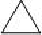
\includegraphics{./Images/Simbolos/simbolo-Almacenamiento-Definitivo.png}
\end{center}
\begin{enumerate}
\item Finanzas: archiva el cheque, el duplicado del recibo, el duplicado del primer Reclamo a Cliente y el triplicado de la factura.
\item Finanzas: archiva el duplicado del primer Reclamo a Cliente, el duplicado del primer y segundo Reclamo a Ventas y el triplicado de la factura.
\item Cliente: archiva el original del recibo.
\item Ventas: almacena copia del segundo y/o tercer Reclamo a Cliente.
\item Legal: almacena copia de Carta Documento.
\end{enumerate}

\pagebreak
\section{Formularios de Cobranzas}
\subsection{Formulario1}
imagen
\begin{itemize}
  \item \textbf{Objetivo:}
  \item \textbf{Alcance:}
  \item \textbf{Emisor:}
  \item \textbf{Cantidad de Copias Emitidas:}
  \item \textbf{Sector receptor:}
 \end{itemize}
\subsubsection{Descripci\'on campos del Formulario1}

\subsection{Formulario2}
imagen
\begin{itemize}
  \item \textbf{Objetivo:}
  \item \textbf{Alcance:}
  \item \textbf{Emisor:}
  \item \textbf{Cantidad de Copias Emitidas:}
  \item \textbf{Sector receptor:}
 \end{itemize}
\subsubsection{Descripci\'on campos del Formulario2}

\pagebreak
\section{Normas de Control Interno de Cobranzas}
